% HW Template for CS 6150, taken from https://www.cs.cmu.edu/~ckingsf/class/02-714/hw-template.tex
%
% You don't need to use LaTeX or this template, but you must turn your homework in as
% a typeset PDF somehow.
%
% How to use:
%    1. Update your information in section "A" below
%    2. Write your answers in section "B" below. Precede answers for all 
%       parts of a question with the command "\question{n}{desc}" where n is
%       the question number and "desc" is a short, one-line description of 
%       the problem. There is no need to restate the problem.
%    3. If a question has multiple parts, precede the answer to part x with the
%       command "\part{x}".
%    4. If a problem asks you to design an algorithm, use the commands
%       \algorithm, \correctness, \runtime to precede your discussion of the 
%       description of the algorithm, its correctness, and its running time, respectively.
%    5. You can include graphics by using the command \includegraphics{FILENAME}
%
\documentclass[11pt]{article}
\usepackage{tikz}
\usetikzlibrary{positioning}
\newdimen\nodeDist
\nodeDist=20mm
\usepackage{amsmath,amssymb,amsthm}
\usepackage{graphicx}
\usepackage[margin=1in]{geometry}
\usepackage{fancyhdr}
\setlength{\parindent}{0pt}
\setlength{\parskip}{5pt plus 1pt}
\setlength{\headheight}{13.6pt}
\newcommand\question[2]{\vspace{.25in}\hrule\textbf{#1: #2}\vspace{.5em}\hrule\vspace{.10in}}
\renewcommand\part[1]{\vspace{.10in}\textbf{(#1)}}
\newcommand\algorithm{\vspace{.10in}\textbf{Algorithm: }}
\newcommand\correctness{\vspace{.10in}\textbf{Correctness: }}
\newcommand\runtime{\vspace{.10in}\textbf{Running time: }}
\pagestyle{fancyplain}
\lhead{\textbf{\NAME\ (\UID)}}
\chead{\textbf{HW\HWNUM}}
\rhead{CS 6150, \today}
\begin{document}\raggedright
%Section A==============Change the values below to match your information==================
\newcommand\NAME{Aishwarya Asesh}  % your name
\newcommand\UID{u1063384}     % your utah UID
\newcommand\HWNUM{1}              % the homework number
%Section B==============Put your answers to the questions below here=======================

% no need to restate the problem --- the graders know which problem is which,
% but replacing "The First Problem" with a short phrase will help you remember
% which problem this is when you read over your homeworks to study.


\question{1}{Solving Recurrences}
Stated Below is the Master Theorem which will be used exaustively in the following answers.
$$T(n) = \left\{ \begin{array}{ll}
                   c             & \mbox{if $n < d$,}\\
                   aT(n/b) + f(n)& \mbox{if $n \geq d$},
                 \end{array}
         \right. $$
where $a \geq 1, b > 1,$ and $d$ are integers and $c$ is a positive
constant.  Let $\nu = \log_b a$.
\begin{description}
\item[Case (i) $f(n)$ is ``definitely smaller'' than $n^\nu$:] If there is a small contant $\epsilon > 0,$ such that 
$f(n) \preceq n^{\nu - \epsilon}$, that is,
$f(n) \prec n^\nu$, then $T(n) \sim n^\nu$.

\item[Case (ii) $f(n)$ is ``similar in size'' to $n^\nu$:] If there is a constant $k \geq 0$, such that 
$f(n) \sim n^{\nu}( \log n)^k$, then 
$T(n) \sim n^{\nu}(\log n)^{k+1}$.

\item[Case (iii) $f(n)$ is ``definitely larger'' than $n^\nu$:] If there are small constants $\epsilon > 0$ and $\delta < 1$, such
that $f(n) \succeq n^{\nu + \epsilon}$ and $a f(n/b) \leq \delta
f(n),$ for $n \geq d$, then $T(n) \sim f(n)$.

\end{description}

\part{a} \textbf{$T(n) = 4T(n/4) + n$.}
\\Here $a=4,b=4,f(n)=n$.
\\ $a,b$ both are greater than 1,
\\Hence applying master theorem: 
\\Compare f(n) with $n^{\log_{b}a}$
\\$n^{log_{b}a}$ = n = $f(n)$. 
\\Condition 2 of Master Method is valid.
\\Therefore, $T(n)=O(n^{\log_{b}a}\log n)$ = $O(n\log n)$

\part{b} $T(n) = 4T(n/4) + 1$.
\\$a,b$ both are greater than 1
\\Hence applying master theorem: 
\\Compare f(n) with $n^{\log_{b}a}$
\\$n^{\log_{b}a}$ = n
\\We know that f(n)=1 which is in the form $O(n^{\log_{4}4-\epsilon})$ where $\epsilon$ is a constant. 
\\Condition 1 for master method holds
\\Hence, T(n)= $O(n^{\log_{4}4})$ = $O(n)$

\part{c} $T(n) = T(n-1) + n$.
\\Solution using Recursion Tree
\\Cost of all subproblem is $C_{n}$, where n is subproblem. 
\\The tree structure is 

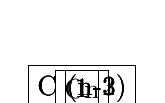
\begin{tikzpicture}[
    node/.style={%
      draw,
      rectangle,
    },
  ]
    \node [node] (A) {Cn};
    \path (A) ++(-115:\nodeDist) node [node] (B) {C (n-1)};
    \path (A) ++(-60:\nodeDist) node [node] (C) {1};
    \path (B) ++(-115:\nodeDist) node [node] (D) {C (n-2)};
    \path (B) ++(-60:\nodeDist) node [node] (E) {1};
    \path (D) ++(-115:\nodeDist) node [node] (F) {C (n-3)};
    \path (D) ++(-60:\nodeDist) node [node] (G) {1};
    \path (F) ++(-115:\nodeDist) node [node] (I) {1};


    \draw (A) -- (B) node [left,pos=0.25] {}(A);
    \draw (A) -- (C) node [right,pos=0.25] {}(A);
    \draw (B) -- (D) node [left,pos=0.25] {}(A);
    \draw (B) -- (E) node [right,pos=0.25] {}(A);
    \draw (D) -- (F) node [left,pos=0.25] {}(A);
    \draw (D) -- (G) node [right,pos=0.25] {}(A);
    \draw [dashed] (F) -- (I) node [right,pos=0.25] {}(A);
\end{tikzpicture}
\\Size of sub prob decreases by 1 at each node
\\depth at which size of subproblem = 1 is 'n'.
\\depth of tree =n
\\Recurrence = Sum of costs at each level =
\\$Cn + C(n-1) + C(n-2) + .........1$
\\$\implies$ n*Cn - e, $\thinspace$ where e = sum of constant terms
\\$\implies$ $Cn^2 - e$
\\$\implies$ $O(n^2)$

\part{d} $T(n) = T(n/3) + T(n/2) + \sqrt{n}$.

Guess: O(n)
\\$T(n)<d(n/3) + d(n/2) + \sqrt{n}$
\\$T(n)<d(5n/6) + \sqrt{n}$
\\$T(n)<Cn + \sqrt{n}$
\\$T(n)<Cn$
\\$T(n)=O(n)$

\part{e} $T(n) = T(\sqrt{n}) + 4$.
\\let m = log n $\implies$ n= $2^m$
\\Replacing n with m
\\$T(2^m)$ = $T(2^m)$ + 1
\\let $T(2^m)$ = S(m)
\\ $S(m) = S(m/2) + 1$
\\Applying Master,
\\$a=1,b=2,f(n)=1$
\\$n^{\log_{b}a}$ = $n^{\log_{2}1}$ = 1 = f(n)
\\Condition 2 holds = 
$ S(m) =O(\log m) = O(\log \log n)$

\part{f} Suppose we have $T(n) = 3T(n/2) + g(n)$.
\\ Analyze the behavior when (a) $g(n) = n^2$ (b) $g(n) = n$, and (c) $g(n) = n^{\log_2 3}$.
\\ For 3 cases: 
\\ Size of subproblem at every level = $n/2^i$, where 'i' denotes level. 
\\ When $\frac{n}{2^i} = 1 $, lets find leaf node
\\$\implies i=\log_{2} n$
\\ levels = $\log_{2} n + 1$
\\ nodes at depth i = $3^i$
\\[10pt] (a) when g(n) =$n^2$
$\implies$ $T(n) = 3T(n/2) + n^2$

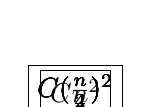
\begin{tikzpicture}[
    node/.style={%
      draw,
      rectangle,
    },
  ]

    \node [node] (A) {$C{n^2}$};
    \path (A) ++(-160:\nodeDist) node [node] (B) {$C(\frac{n}{2})^2$};
    \path (A) ++(-50:\nodeDist) node [node] (C) {$C(\frac{n}{2})^2$};
    \path (A) ++(-10:\nodeDist) node [node] (D) {$C(\frac{n}{2})^2$};
    \path (B) ++(-160:\nodeDist) node [node] (E) {$C(\frac{n}{4})^2$};
    \path (B) ++(-100:\nodeDist) node [node] (F) {$C(\frac{n}{4})^2$};
    \path (B) ++(-40:\nodeDist) node [node] (G) {$C(\frac{n}{4})^2$};
    
    \draw (A) -- (B) node [left,pos=0.25] {}(A);
    \draw (A) -- (C) node [right,pos=0.25] {}(A);
    \draw (A) -- (D) node [left,pos=0.25] {}(A);
    \draw (B) -- (E) node [right,pos=0.25] {}(A);
    \draw (B) -- (F) node [left,pos=0.25] {}(A);
    \draw (B) -- (G) node [right,pos=0.25] {}(A);
    \end{tikzpicture}
\\ 
Cost of a subproblem at each level = $(\frac{n}{2^i})^2$
\\ Cost = each level= $3^i(\frac{n}{2^i})^2 = (\frac{3}{4})^i*n^2)$
\\ $Cost$ = leaf node = $3^i = 3^{\log n} = n^{log_{2} 3}$, where leaf = T(1) to the cost. So cost at level $\log n$ is $\theta (n^{log_{2} 3})$.
\\ T(n) = $cn^2 + \frac{3}{4} cn^2+\frac{9}{16} cn^2+ ....+(\frac{3}{4})^{log_{2} (n-1)} cn^2 + \theta(n^{log_{2} 3})$
\\Infinite GP case:
\\$T(n) <  \frac{cn^2}{1-\frac{3}{4}}$+$\theta (n^{\log_{2} 3})$
\\$\implies \mathcal{O}(n^2).$
\\ Condition 3 of the Master Theorem:
\\[10pt] (b) when g(n) =$n$
$\implies$ $T(n) = 3T(n/2) + n$

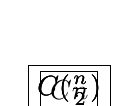
\begin{tikzpicture}[
    node/.style={%
      draw,
      rectangle,
    },
  ]

    \node [node] (A) {$C{n}$};
    \path (A) ++(-160:\nodeDist) node [node] (B) {$C(\frac{n}{2})$};
    \path (A) ++(-50:\nodeDist) node [node] (C) {$C(\frac{n}{2})$};
    \path (A) ++(-10:\nodeDist) node [node] (D) {$C(\frac{n}{2})$};
    
    \draw (A) -- (B) node [left,pos=0.25] {}(A);
    \draw (A) -- (C) node [right,pos=0.25] {}(A);
    \draw (A) -- (D) node [left,pos=0.25] {}(A);
    \end{tikzpicture}
\\ 
Cost of a subproblem = $(\frac{n}{2^i})$
\\ Cost = each level= $3^{i(\frac{n}{2^i})} = (\frac{3}{2})^{i*n})$
\\ Cost = leaf node = $3^i = 3^{log n} = n^{log_{2} 3}$, where leaf = T(1) to the cost. So cost at level log n is $\theta (n^{log_{2} 3})$.
\\$\implies T(n) = \mathcal{O} (n^{\log_{2} 3})$
\\Condition 1 of the Master Theorem:
\\[10pt] (c) when g(n) =$n^{\log_{2} 3}$
$\implies$ $T(n) = 3T(n/2) + n^{\log_{2} 3}$

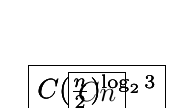
\begin{tikzpicture}[
    node/.style={%
      draw,
      rectangle,
    },
  ]

    \node [node] (A) {$C{n}$};
    \path (A) ++(-160:\nodeDist) node [node] (B) {$C(\frac{n}{2})^{\log_{2}3}$};
    \path (A) ++(-50:\nodeDist) node [node] (C) {$C(\frac{n}{2})^{\log_{2}3}$};
    \path (A) ++(-10:\nodeDist) node [node] (D) {$C(\frac{n}{2})^{\log_{2}3}$};
    
    \draw (A) -- (B) node [left,pos=0.25] {}(A);
    \draw (A) -- (C) node [right,pos=0.25] {}(A);
    \draw (A) -- (D) node [left,pos=0.25] {}(A);
    \end{tikzpicture}
 
Cost = leaf node =$ 3^i = 3^{log n} = n^{log_{2} 3}$, where leaf = T(1) to the cost. So cost at level $log n$ is $\theta (n^{log_{2} 3}).$
\\ T(n) = $cn^{log_{2} 3} + \frac{3}{2} cn^{log_{2} 3}+\frac{9}{4} cn^{log_{2} 3}+ ....+(\frac{3}{2})^{log_{2} n-1} cn^{log_{2} 3} + \theta(n^{log_{2} 3})$
\\T(n) $= (n^{log_{2} 3})\sum_{j=0}^{logn -1}$ $(\frac{3}{2})^{log_{2} 3}$
\\T(n) = $\mathcal{O}(n^{2(\log_{2} 3)} \log n)$
\\Condition 2 of the Master Theorem.

\question{2}{Sorting "nearby'' numbers} 

\algorithm The given case can be solved using the concept of Counting Sort. The first step is to scan through the array to determine the minimum and the maximum element. Let B be a new array of size M created that has each value as a constant 0. The array is scanned again and for each number in A[i], we increment $B[min_{i}\{A[i]\} + A[i]]$. A new array C[0..n-1] is created. In the final step we scan through the array B[] and for each number B[i], we can place B[i] values of i into the coming B[i] null slots of C[].
\\Thus we count the exact time value i occurs in the array and store the data in B[i]. We get the sorted array when we scan through B[i] and get the values in order.
  
\correctness All the elements of A[] is stored in C[] in sorted order. So accuracy is 100\%

\runtime During the scan process, we scan the elements of array with sizes 'n' and 'M' regularly, so it takes $O(n + M)$ times.

\question{3}{Selecting in an Union}
\algorithm Check the sum of middle index of array A and B.
\\$if$ $sum<k$ and $middle$ $element$ $of$ $k>middle$ element $of$ B
\\discard the first half of B and new value of k =$K - (index$ of $mid-elem$ of $B)-1$
\\$else$ $if$
\\mid-elem of B is greater
\\discard the first half of A and new value of $k =K - (index$ of $mid-elem$ of $A)-1$
\\repeat till length of $A$ or $B$ is zero.\\
\correctness We get the desired kth smallest element using the abve steps, thus we have the $100\% $ correctness.

\runtime In every repetition, we are performing computations on middle half of list, and based on if-else we remove half list in one of the array. Thus this dividing process takes $O(log n)$ time complexity.

\question{4}{Closest Pair}

\part{a}
Let the instances be 1,3,8 separated by an imaginary axis with instances 9,15,19. Now if we try to find the smallest distance, it comes as 4 between 15 and 19 and 2 between 1 and 3. So the closest distance is considered as 2. But actually points 8 and 9 are separated by just a point distance. So the consideration goes wrong in this case.
\\
\part{b} 
Steps for proof:
\\We will consider a square.
\\We need to show that any 2 points are at a minimum distance d.
\\Let us consider a square area.
\\Let a point be placed on any corner.
\\The next point cannot be placed any where other than the other remaining vertices of the square.
\\Thus this way we get 4 different points placed on the vertices of the square area.
\\If we consider any 5th point, the distance of 5th point from other 4 points will be strictly smaller than d.
\\Thus proved.

\part{c} Steps involved and time computations:
\\finding median x = O(n)
\\recurse the two sub probs of size $n/2$  = 2T(n/2)
\\discard points = O(n)
\\$sort$ y values = $O(n \log n)$
\\iterate thorugh a list of y variables and computation for each = O(n)
\\Thus total = \[ T(n) = 2T(n/2) + O(n \log n). \]
For bound -
\[ T(n) = 2T(n/2) + O(n \log n). \]
\[ T(n) = \Sigma_{i=1}^m + \Sigma_{i=1}^m \log(n/2^{i-1}) + {where } (m) = log n\] 
\[ T(n) <= O(2^{\log n}) + O(n(log n + log (n/2) + log(n/4) + ...... + 1) \]
\[ T(n) <= O(n) + O(n log(log n)) \]
\[ T(n) <= O(n log^2 n) \]

\question{5}{Linear Time Median}
\part{a} Using the recursive formula we know that $T(n)=O(n) + T(n/5) + T(7n/10)$
\\We assume that $T(n) = (a*n) + T(n/5) + T(7n/10)$
\\$C*n>=T(n/5) + T(7n/10) +a*n$
\\$C*n>=C*n/5 + C*7n/10 +a*n$
\\$C>9*C/10 + a$
\\$C/10 >= a$ 
\\$C>=10*a$
\\so T(n)= O(n)
\\Here if we divide the group into 3 then:
\\$T(n)=O(n) + T(n/3) + T(2n/3) so T(n) > O(n)...$
\\if groups are divided into more than 5, Value of constant 5 is more,so that is the most optimal solution.
\\In which case running time is $T_{median}(n/5) + O(n)$ 
\\[10pt]
\part{b} Recurrence for finding the near median is $T(N) \leq T(N/S) + T(B/N) +O(N)$ as we see,
\\$T(N/S)$ = cost of finding median of $A_{medians}$ and N is the cost of partitioning algo.
\\$T(B/N)$ = cost of final recursive call
\\$B$ = fraction of $(BN)$ i.e. worst case length of either $A_{l}$ $A_{r}$
\\$M$ = median of $A_{medians}$
\\$M$ must = $1/2(N/5)$ except the median itself, not including 5 elements from last median cluster.
\\$G-2$ = $1/2(N/5)$
\\now at least 3 elements are smaller or equal to $M$
\\$3(G-2) = 1/2(N/5)$ i.e $(3N/10) - 9 \geqslant N/4$
\\This proves the algo. 

\end{document}
